\documentclass{article}

\usepackage{graphicx, xcolor}
\usepackage{amsmath, amssymb}
\usepackage{subcaption}
\usepackage{float}
\usepackage[colorlinks=true,allcolors=blue]{hyperref}

\usepackage[margin=1in]{geometry}

\def\hwtitle{Homework 9: Metropolis algorithm and the canonical ensemble}
\def\hwauthor{Caden Gobat}
\def\hwdate{April 21, 2021}

\usepackage{fancyhdr}
\lhead{\hwauthor}
\chead{\hwtitle}
\rhead{\hwdate}
\lfoot{\hwauthor}
\cfoot{}
\rfoot{\thepage}
\renewcommand{\footrulewidth}{0.4pt}
\pagestyle{fancy}

\author{\hwauthor}
\title{\hwtitle}
\date{\hwdate}

\begin{document}

\maketitle
\thispagestyle{fancy}

\section{Introduction}

Last week, we made a foray into molecular dynamics by implementing an $N$-body simulation of gas particles interacting via only the Lennard-Jones potential: \begin{equation}
   V(r)=4\epsilon\left[\left(\frac{r_0}{r}\right)^{12} - \left(\frac{r_0}{r}\right)^6\right]
\end{equation}

This was the microcanonical ensemble. Now we will use the Metropolis algorithm to simulate the canonical ensemble by accepting or rejecting randomly chosen updates based on a probability which is dependent on the partition function of the system. The probability distribution of microstates is given by \begin{equation}
   P(s)=\frac{1}{Z}e^{\frac{-1}{kT}E(s)}
\end{equation}
where $\displaystyle E(s)=\frac{1}{2}\sum_{i=1}^{N} v_{i}^2 + \sum_{i=1}^{N} \sum_{j=i+1}^{N} V(r_{ij})$. We have now transitioned to using the \emph{canonical} ensemble, because here we hold $kT$ constant, rather than $E$.

\section{Results}

\bigskip
\noindent{\bf Question 1}
\medskip

A snapshot of the first system ($kT=0.5$) is shown in Fig.~\ref{fig:kT0.5}. This setup takes approximately 2000 steps to thermalize, and the conditions to reach an approximately 50\% acceptance rate are $dx=0.14$ and $dv=0.14$. The second system ($kT=5$) is shown in Fig.~\ref{fig:kT5.0}. It takes around 300 steps to thermalize, and the parameters that lead to 50\% acceptance here are $dx=2.2$ and $dv=2.2$. This is an increase by a factor of $\frac{2.2}{0.14}\cong15.7$, which is as expected, because we increased temperature by a factor of 10, so we expect these values to increase by a factor of $\frac{3}{2}\Delta kT=\frac{3}{2}(10)=15$.

\begin{figure}[H]
\centering
\begin{subfigure}{.5\textwidth}
  \centering
  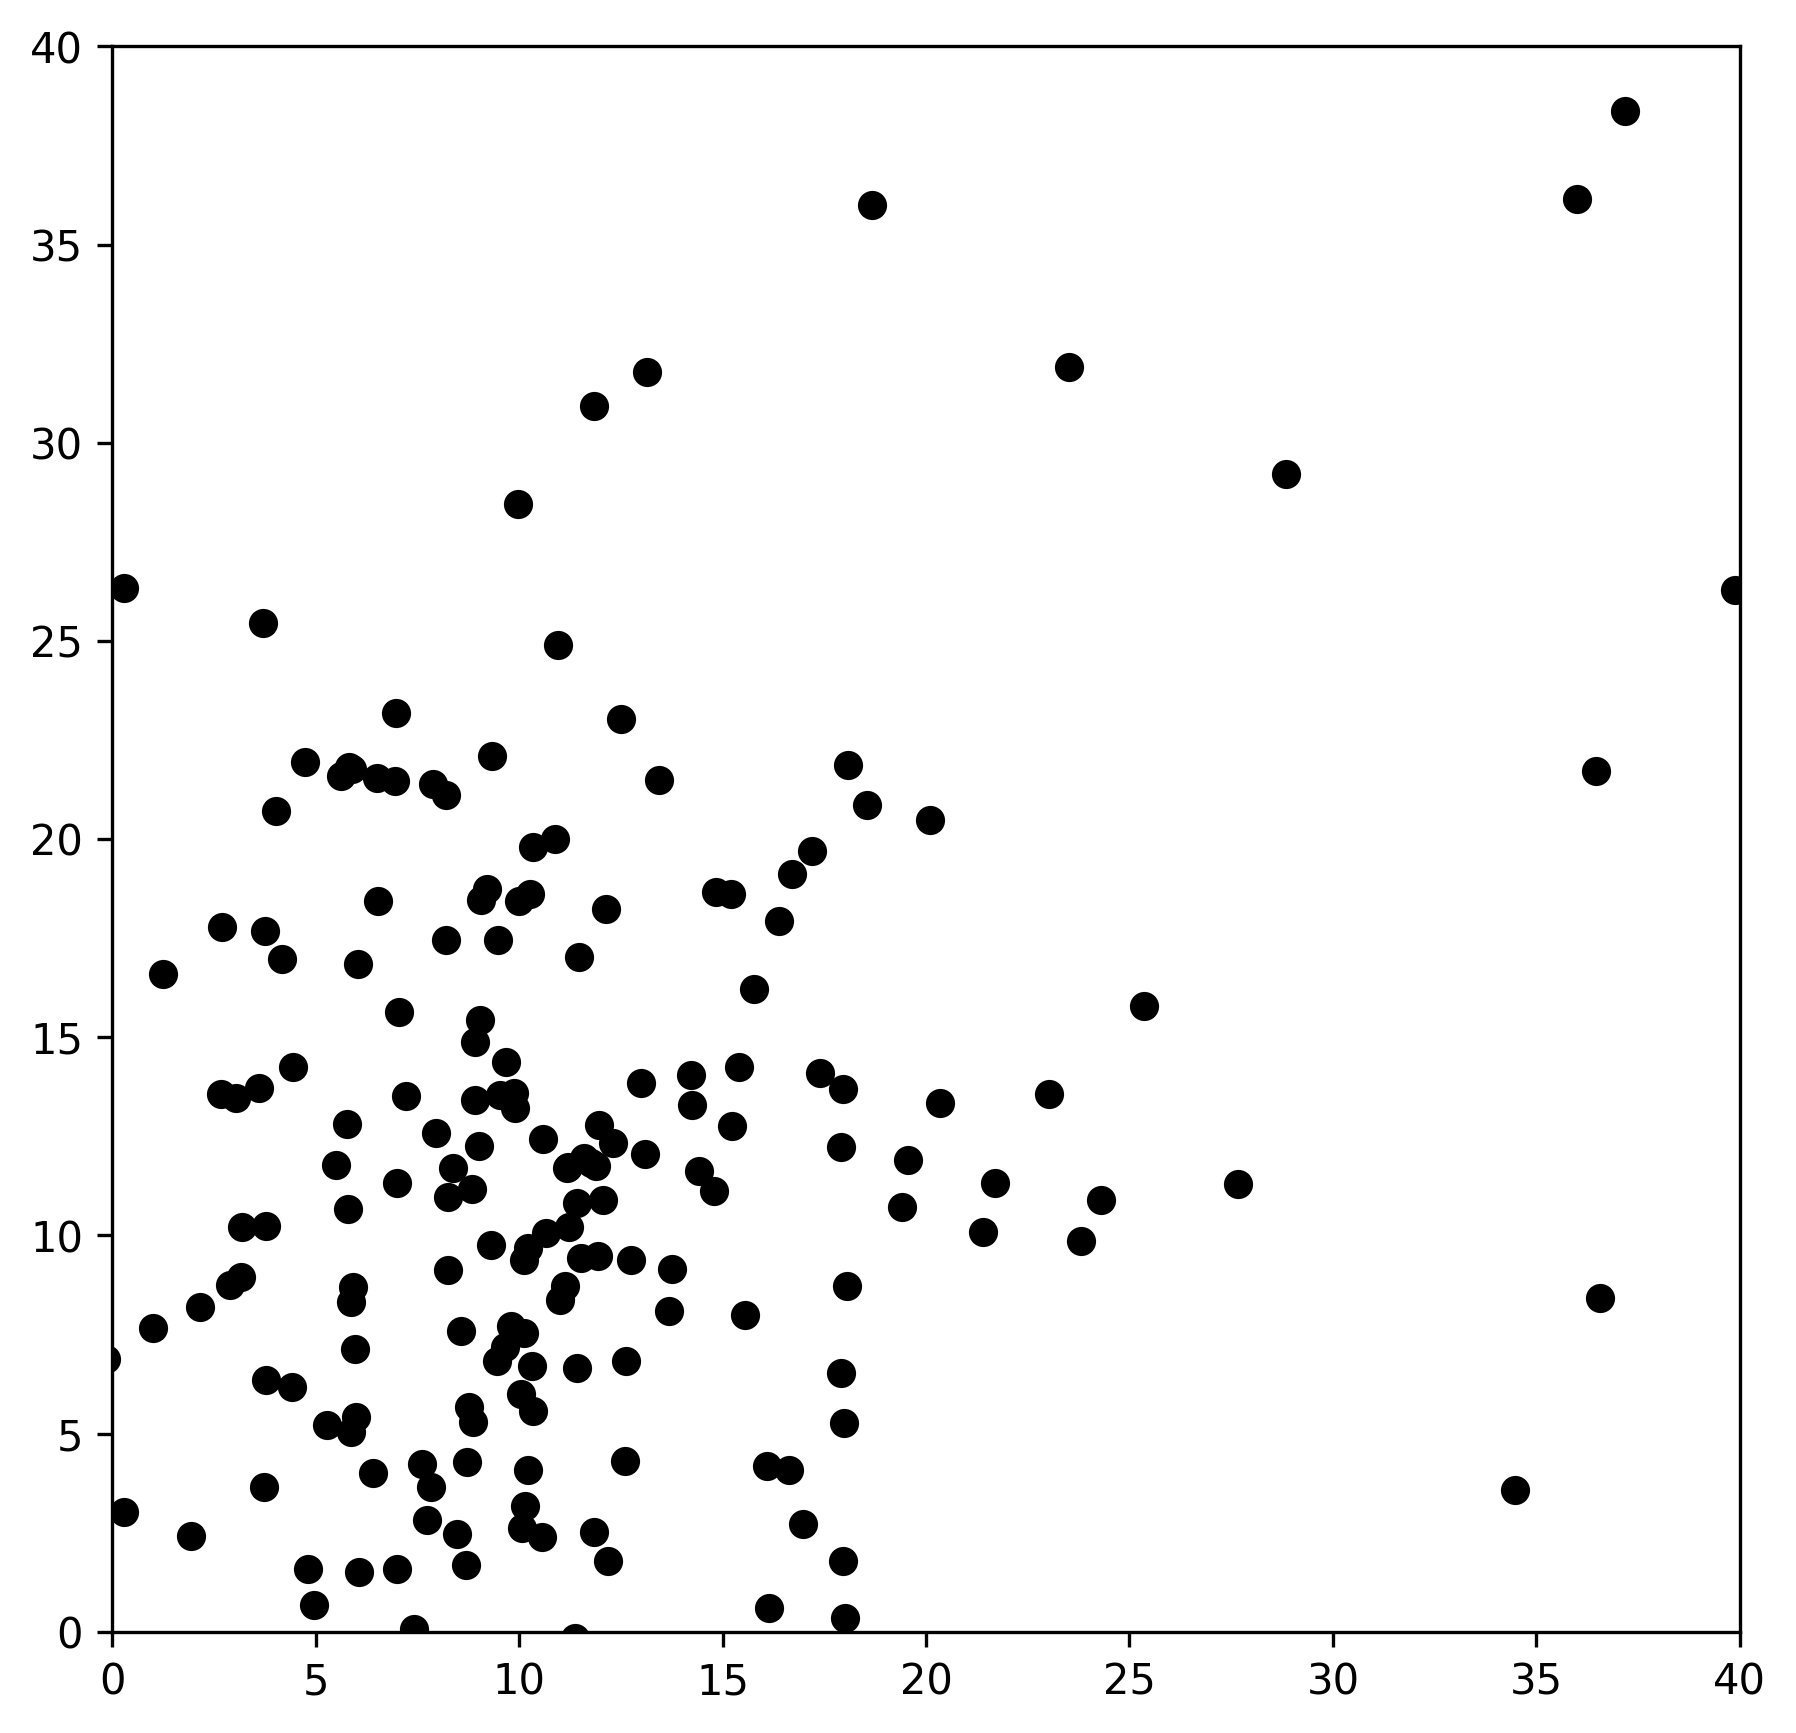
\includegraphics[width=.9\linewidth]{homework9/1a.png}
  \caption{$kT=0.5$.}
  \label{fig:kT0.5}
\end{subfigure}%
\begin{subfigure}{.5\textwidth}
  \centering
  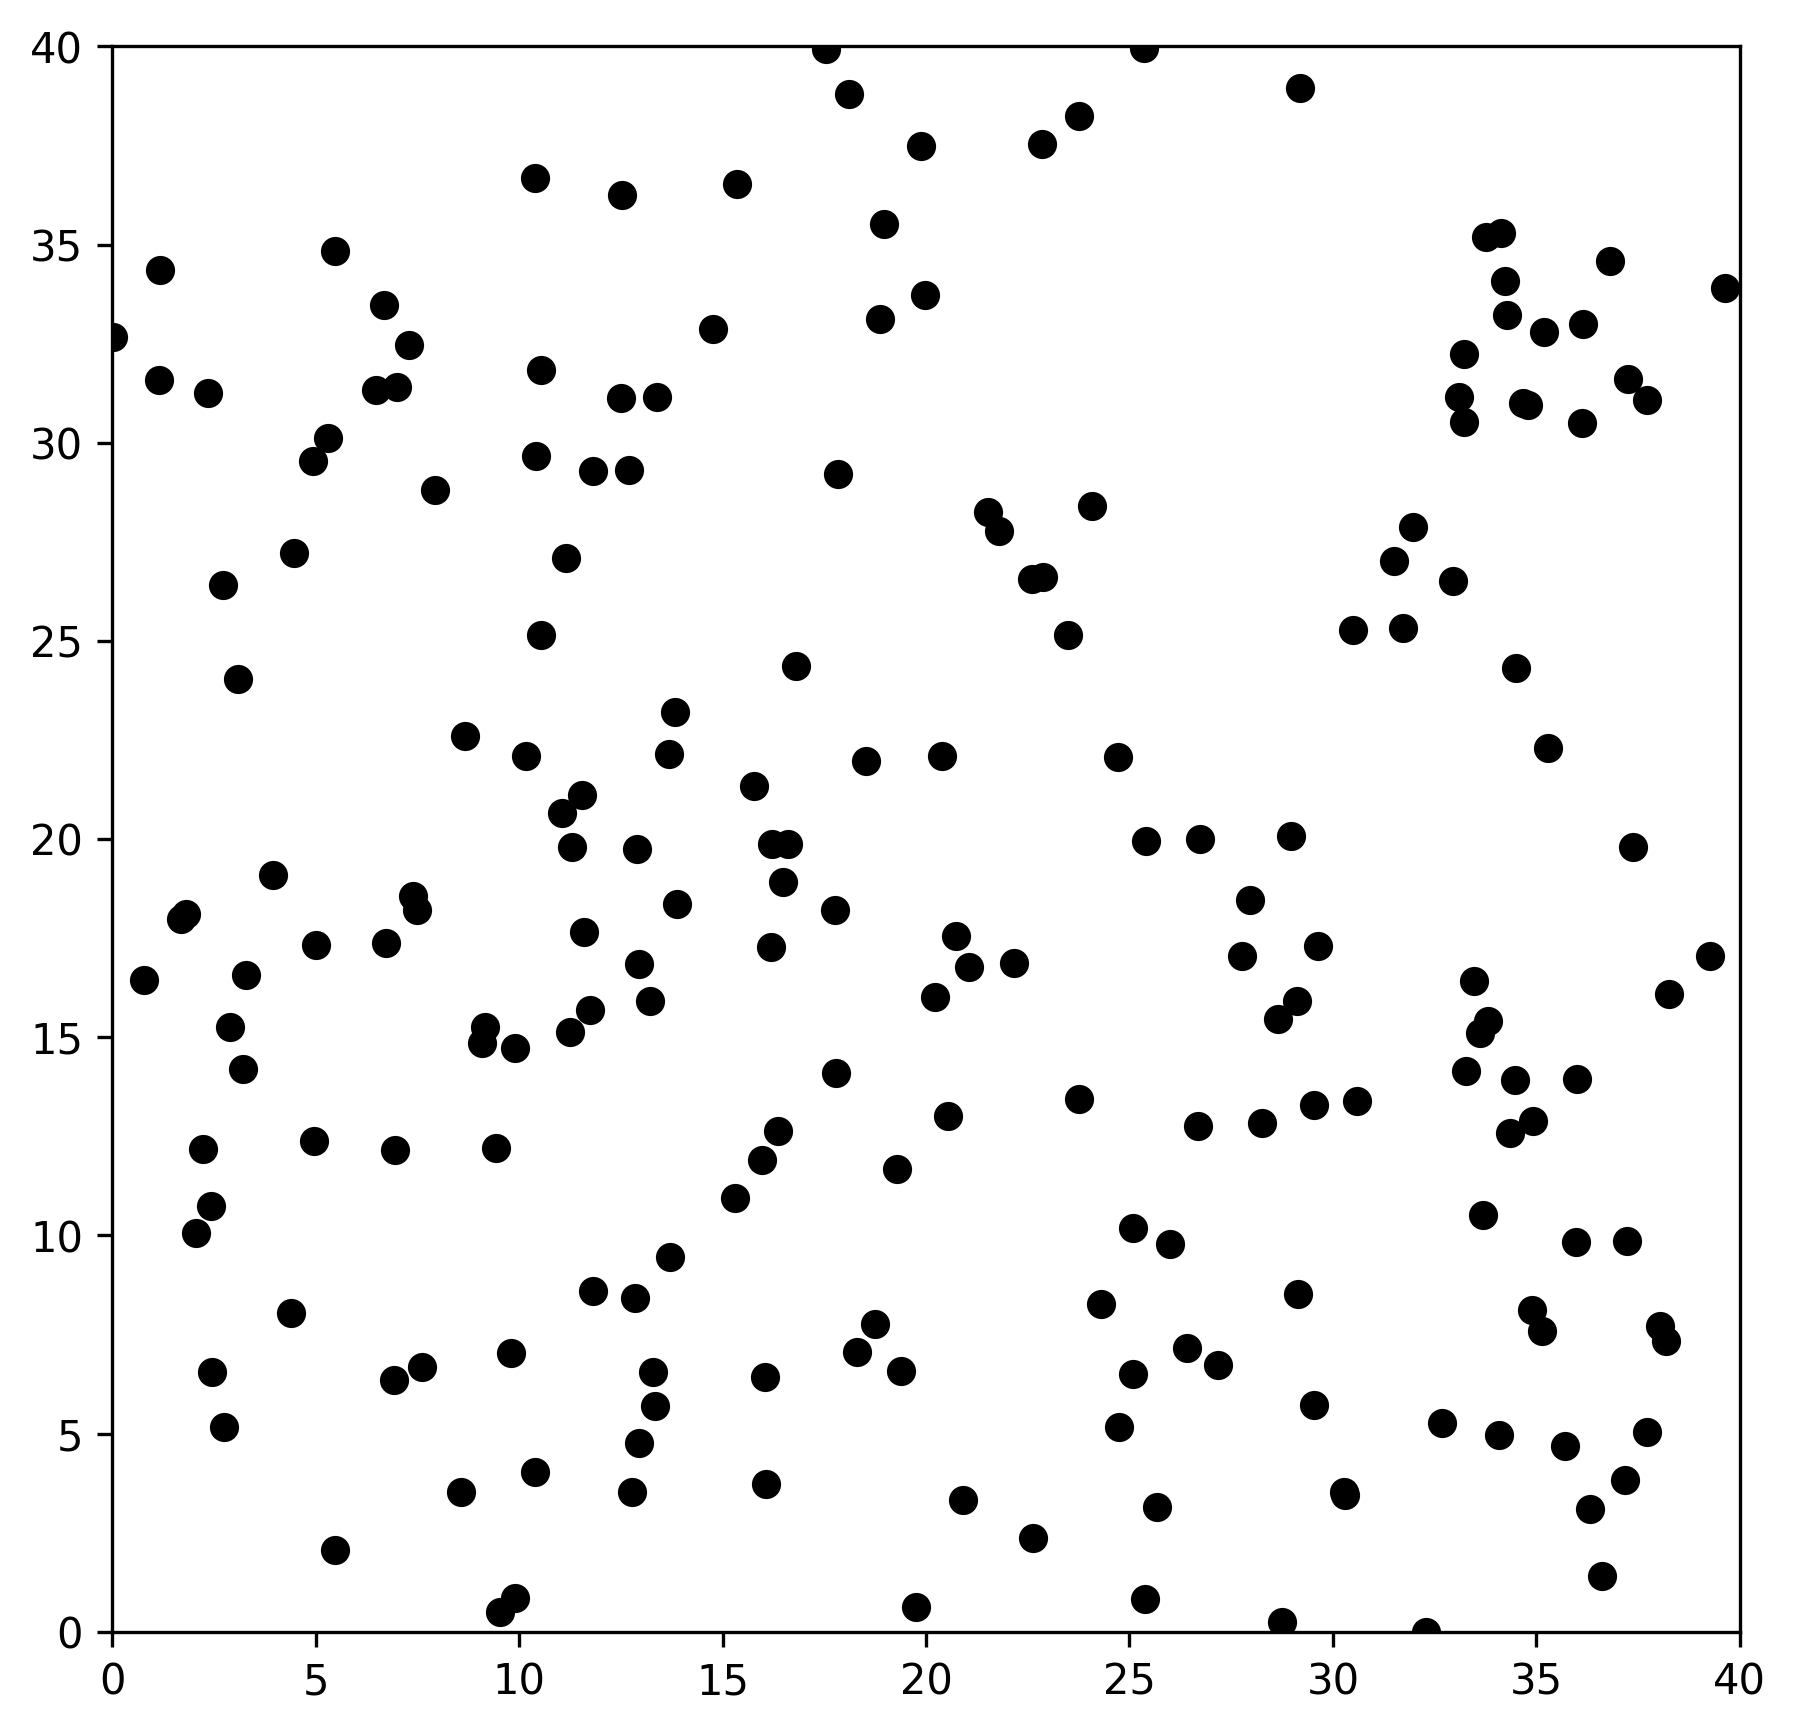
\includegraphics[width=.9\linewidth]{homework9/1b.png}
  \caption{$kT=5$.}
  \label{fig:kT5.0}
\end{subfigure}
\caption{Representative microstate snapshots of the system: $N=200$, $L=40$.}
\label{fig:p1}
\end{figure}

\bigskip
\noindent{\bf Question 2}
\medskip

\begin{figure}[H]
    \centering
    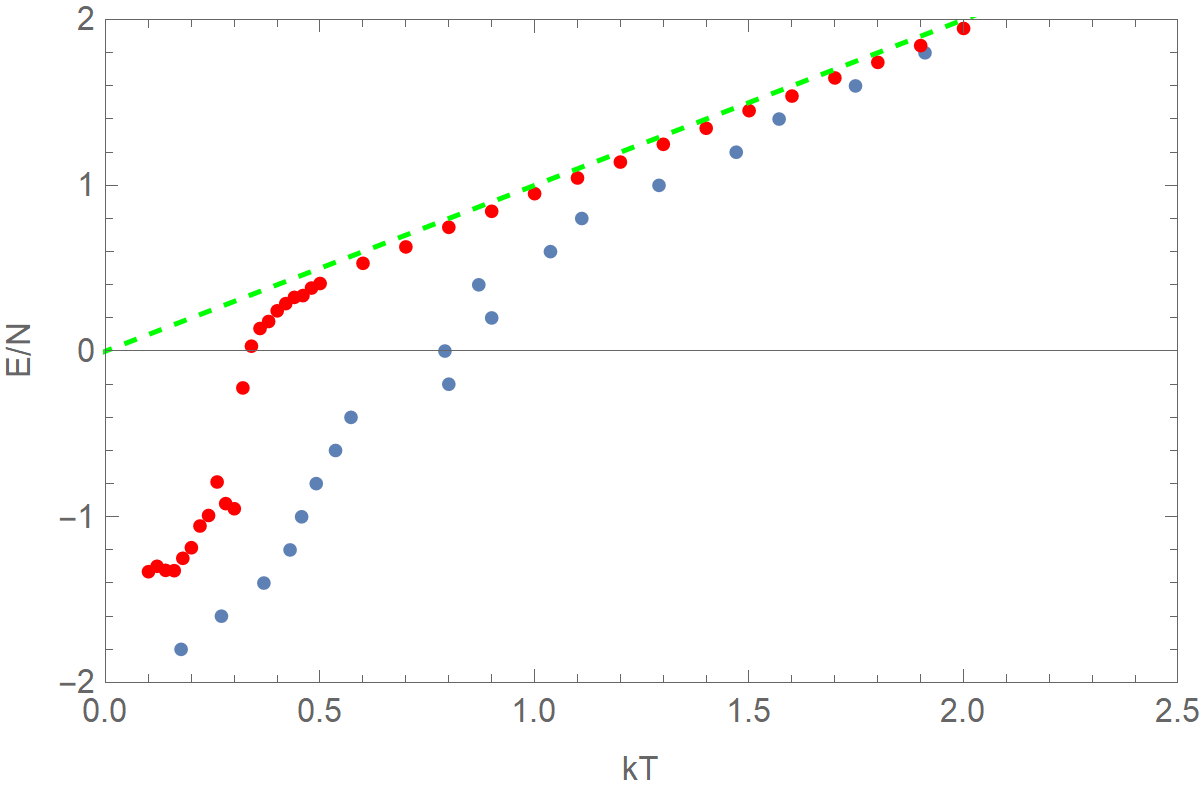
\includegraphics[width=0.7\textwidth]{homework9/p2.png}
    \caption{Relationship between particle energy and temperature for a system with $N=20$ and $L=40$. In red, $\langle E \rangle /N$ as a function of $kT$ values from 0.1 to 0.5 in steps of 0.02 and from 0.5 to 2 in steps of 0.1 (canonical). In blue, $kT$ computed using last week's code as a function of $E/N$ in the range $-1.8$ to $1.8$ in steps of 0.2 (microcanonical). The relationship between these two variables for an ideal has is shown as the dashed green line. Both simulations get closer to reflecting the ideal gas relationship at higher values of $E/N$ and $kT$. More points in the canonical model are closer to the green line, but it also deviates more sharply below the transition point (somewhere around $kT\cong0.25$, from visual inspection). In general, the microcanonical result behaves similarly, but approaches the ideal gas curve much more gradually, without such a sharp transition.}
    \label{fig:p2}
\end{figure}

\bigskip
\noindent{\bf Question 3}
\medskip

\begin{figure}[H]
    \centering
    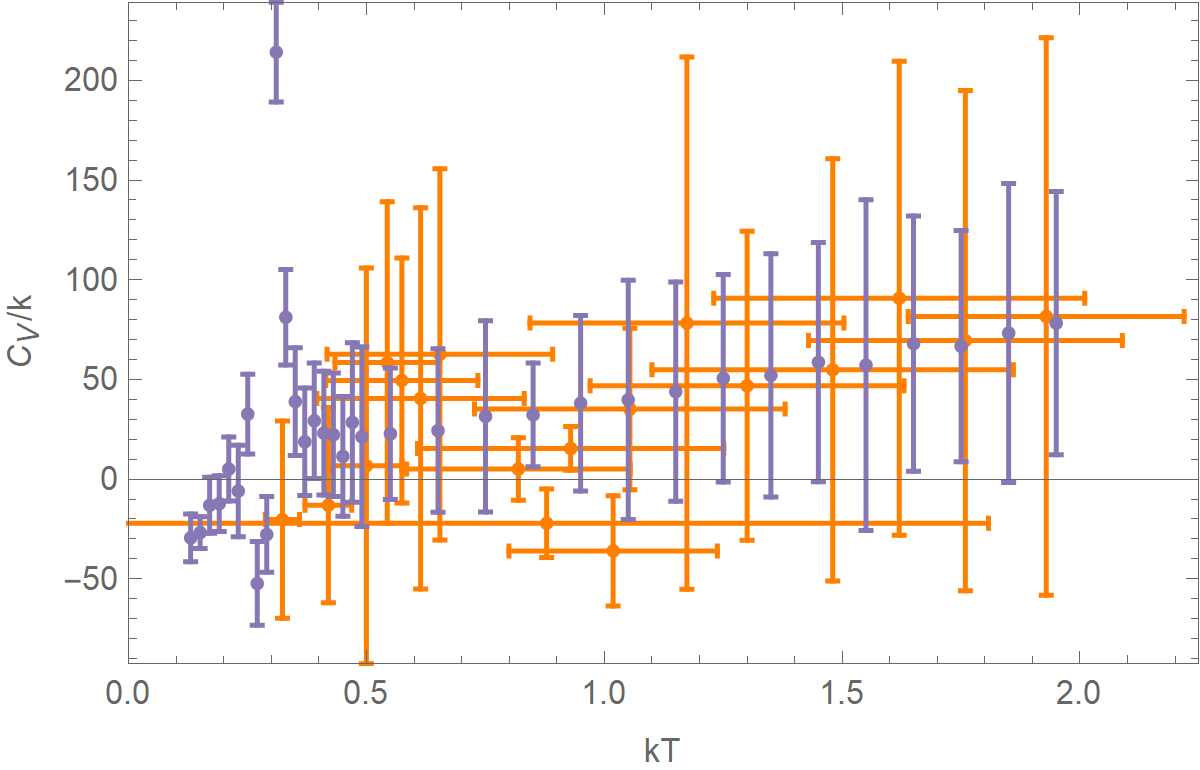
\includegraphics[width=.7\textwidth]{homework9/p3.png}
    \caption{Plot of specific heat as a function of temperature, calculated using two methods. In purple, the specific heat is calculated by interpolating the red data in Fig.~\ref{fig:p2} using Eq.~\ref{eq:derivative}. In orange, specific heat and temperature calculated using the variance in energy (as in Eq.~\ref{eq:variance}). The first method, which also corresponds to a canonical approach to the problem, provides a much cleaner result, with the peak at the transition temperature being clearly visible and the error bars being much more manageable. From this we can determine that the transition temperature is around $kT\cong0.3$. While it does not immediately clear from this plot whether the ideal gas prediction of $\displaystyle\lim_{kT\to\infty}C_V/k = N$ will hold, $C_V/k=N=20$ is within the error for most of the points here.}
    \label{fig:p3}
\end{figure}

Two methods for calculating specific heat:
\begin{equation}\label{eq:derivative}
    C_V/k \approx \frac{\langle E \rangle (kT+\delta/2)-\langle E \rangle (kT-\delta/2)}{\delta}
\end{equation}

\begin{equation}\label{eq:variance}
    C_V/k = \frac{\langle E^2 \rangle - \langle E\rangle^2}{(kT)^2}
\end{equation}

\section{Conclusions}

The contrast between this project and our work in the previous one was very interesting to me. Although both address the same fundamental problem, the difference in algorithms between Metropolis and direct numerical RK2 integration yields some interesting results, and are really quite different from a computational perspective. Yet again I was very intrigued by the appearance of many of the concepts and terminology we have learned in Thermal \& Statistical Physics, and seeing some of the same main results arise from computational methods as from analytical derivations was gratifying.


\end{document}
